\documentclass[1p]{elsarticle_modified}
%\bibliographystyle{elsarticle-num}

%\usepackage[colorlinks]{hyperref}
%\usepackage{abbrmath_seonhwa} %\Abb, \Ascr, \Acal ,\Abf, \Afrak
\usepackage{amsfonts}
\usepackage{amssymb}
\usepackage{amsmath}
\usepackage{amsthm}
\usepackage{scalefnt}
\usepackage{amsbsy}
\usepackage{kotex}
\usepackage{caption}
\usepackage{subfig}
\usepackage{color}
\usepackage{graphicx}
\usepackage{xcolor} %% white, black, red, green, blue, cyan, magenta, yellow
\usepackage{float}
\usepackage{setspace}
\usepackage{hyperref}

\usepackage{tikz}
\usetikzlibrary{arrows}

\usepackage{multirow}
\usepackage{array} % fixed length table
\usepackage{hhline}

%%%%%%%%%%%%%%%%%%%%%
\makeatletter
\renewcommand*\env@matrix[1][\arraystretch]{%
	\edef\arraystretch{#1}%
	\hskip -\arraycolsep
	\let\@ifnextchar\new@ifnextchar
	\array{*\c@MaxMatrixCols c}}
\makeatother %https://tex.stackexchange.com/questions/14071/how-can-i-increase-the-line-spacing-in-a-matrix
%%%%%%%%%%%%%%%

\usepackage[normalem]{ulem}

\newcommand{\msout}[1]{\ifmmode\text{\sout{\ensuremath{#1}}}\else\sout{#1}\fi}
%SOURCE: \msout is \stkout macro in https://tex.stackexchange.com/questions/20609/strikeout-in-math-mode

\newcommand{\cancel}[1]{
	\ifmmode
	{\color{red}\msout{#1}}
	\else
	{\color{red}\sout{#1}}
	\fi
}

\newcommand{\add}[1]{
	{\color{blue}\uwave{#1}}
}

\newcommand{\replace}[2]{
	\ifmmode
	{\color{red}\msout{#1}}{\color{blue}\uwave{#2}}
	\else
	{\color{red}\sout{#1}}{\color{blue}\uwave{#2}}
	\fi
}

\newcommand{\Sol}{\mathcal{S}} %segment
\newcommand{\D}{D} %diagram
\newcommand{\A}{\mathcal{A}} %arc


%%%%%%%%%%%%%%%%%%%%%%%%%%%%%5 test

\def\sl{\operatorname{\textup{SL}}(2,\Cbb)}
\def\psl{\operatorname{\textup{PSL}}(2,\Cbb)}
\def\quan{\mkern 1mu \triangleright \mkern 1mu}

\theoremstyle{definition}
\newtheorem{thm}{Theorem}[section]
\newtheorem{prop}[thm]{Proposition}
\newtheorem{lem}[thm]{Lemma}
\newtheorem{ques}[thm]{Question}
\newtheorem{cor}[thm]{Corollary}
\newtheorem{defn}[thm]{Definition}
\newtheorem{exam}[thm]{Example}
\newtheorem{rmk}[thm]{Remark}
\newtheorem{alg}[thm]{Algorithm}

\newcommand{\I}{\sqrt{-1}}
\begin{document}

%\begin{frontmatter}
%
%\title{Boundary parabolic representations of knots up to 8 crossings}
%
%%% Group authors per affiliation:
%\author{Yunhi Cho} 
%\address{Department of Mathematics, University of Seoul, Seoul, Korea}
%\ead{yhcho@uos.ac.kr}
%
%
%\author{Seonhwa Kim} %\fnref{s_kim}}
%\address{Center for Geometry and Physics, Institute for Basic Science, Pohang, 37673, Korea}
%\ead{ryeona17@ibs.re.kr}
%
%\author{Hyuk Kim}
%\address{Department of Mathematical Sciences, Seoul National University, Seoul 08826, Korea}
%\ead{hyukkim@snu.ac.kr}
%
%\author{Seokbeom Yoon}
%\address{Department of Mathematical Sciences, Seoul National University, Seoul, 08826,  Korea}
%\ead{sbyoon15@snu.ac.kr}
%
%\begin{abstract}
%We find all boundary parabolic representation of knots up to 8 crossings.
%
%\end{abstract}
%\begin{keyword}
%    \MSC[2010] 57M25 
%\end{keyword}
%
%\end{frontmatter}

%\linenumbers
%\tableofcontents
%
\newcommand\colored[1]{\textcolor{white}{\rule[-0.35ex]{0.8em}{1.4ex}}\kern-0.8em\color{red} #1}%
%\newcommand\colored[1]{\textcolor{white}{ #1}\kern-2.17ex	\textcolor{white}{ #1}\kern-1.81ex	\textcolor{white}{ #1}\kern-2.15ex\color{red}#1	}

{\Large $\underline{12a_{0610}~(K12a_{0610})}$}

\setlength{\tabcolsep}{10pt}
\renewcommand{\arraystretch}{1.6}
\vspace{1cm}\begin{tabular}{m{100pt}>{\centering\arraybackslash}m{274pt}}
\multirow{5}{120pt}{
	\centering
	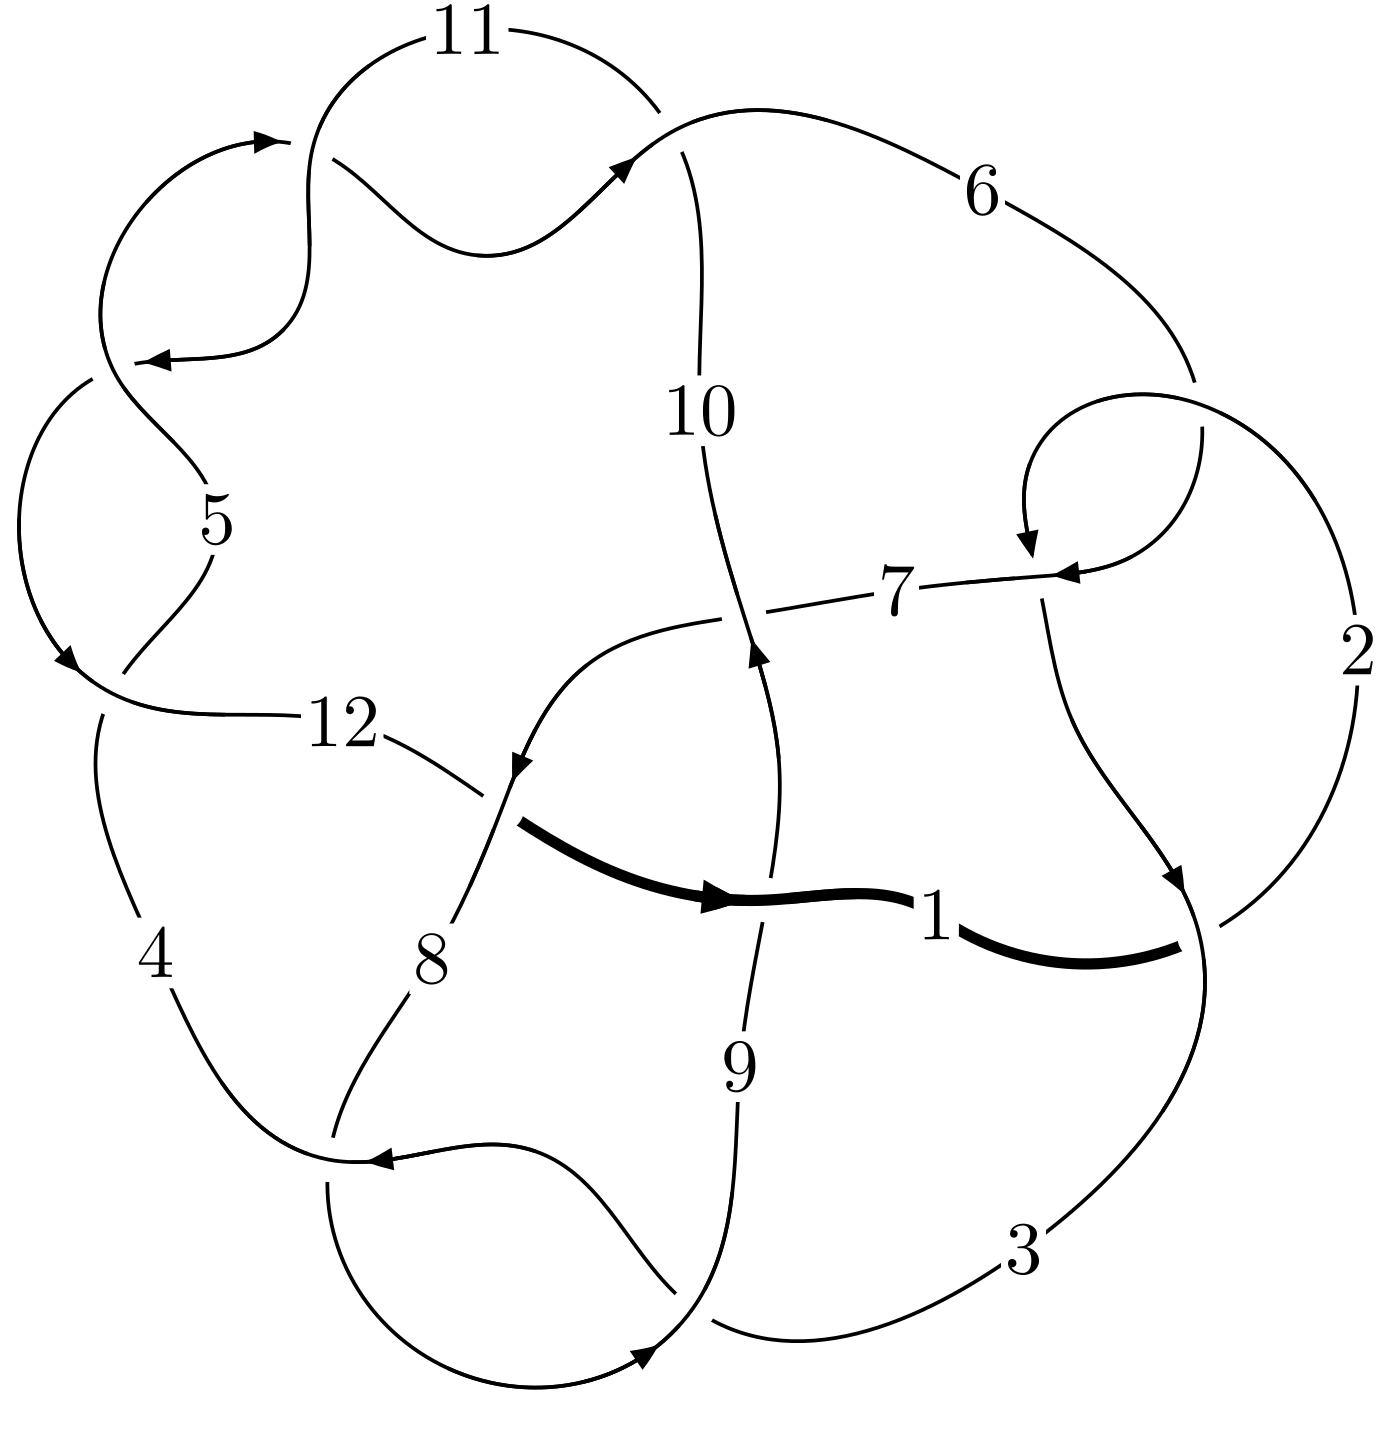
\includegraphics[width=112pt]{../../../GIT/diagram.site/Diagrams/png/1411_12a_0610.png}\\
\ \ \ A knot diagram\footnotemark}&
\allowdisplaybreaks
\textbf{Linearized knot diagam} \\
\cline{2-2}
 &
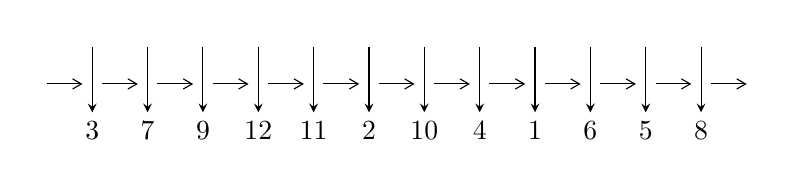
\begin{tikzpicture}[x=20pt, y=17pt]
	% nodes
	\node (C0) at (0, 0) {};
	\node (C1) at (1, 0) {};
	\node (C1U) at (1, +1) {};
	\node (C1D) at (1, -1) {3};

	\node (C2) at (2, 0) {};
	\node (C2U) at (2, +1) {};
	\node (C2D) at (2, -1) {7};

	\node (C3) at (3, 0) {};
	\node (C3U) at (3, +1) {};
	\node (C3D) at (3, -1) {9};

	\node (C4) at (4, 0) {};
	\node (C4U) at (4, +1) {};
	\node (C4D) at (4, -1) {12};

	\node (C5) at (5, 0) {};
	\node (C5U) at (5, +1) {};
	\node (C5D) at (5, -1) {11};

	\node (C6) at (6, 0) {};
	\node (C6U) at (6, +1) {};
	\node (C6D) at (6, -1) {2};

	\node (C7) at (7, 0) {};
	\node (C7U) at (7, +1) {};
	\node (C7D) at (7, -1) {10};

	\node (C8) at (8, 0) {};
	\node (C8U) at (8, +1) {};
	\node (C8D) at (8, -1) {4};

	\node (C9) at (9, 0) {};
	\node (C9U) at (9, +1) {};
	\node (C9D) at (9, -1) {1};

	\node (C10) at (10, 0) {};
	\node (C10U) at (10, +1) {};
	\node (C10D) at (10, -1) {6};

	\node (C11) at (11, 0) {};
	\node (C11U) at (11, +1) {};
	\node (C11D) at (11, -1) {5};

	\node (C12) at (12, 0) {};
	\node (C12U) at (12, +1) {};
	\node (C12D) at (12, -1) {8};
	\node (C13) at (13, 0) {};

	% arrows
	\draw[->,>={angle 60}]
	(C0) edge (C1) (C1) edge (C2) (C2) edge (C3) (C3) edge (C4) (C4) edge (C5) (C5) edge (C6) (C6) edge (C7) (C7) edge (C8) (C8) edge (C9) (C9) edge (C10) (C10) edge (C11) (C11) edge (C12) (C12) edge (C13) ;	\draw[->,>=stealth]
	(C1U) edge (C1D) (C2U) edge (C2D) (C3U) edge (C3D) (C4U) edge (C4D) (C5U) edge (C5D) (C6U) edge (C6D) (C7U) edge (C7D) (C8U) edge (C8D) (C9U) edge (C9D) (C10U) edge (C10D) (C11U) edge (C11D) (C12U) edge (C12D) ;
	\end{tikzpicture} \\
\hhline{~~} \\& 
\textbf{Solving Sequence} \\ \cline{2-2} 
 &
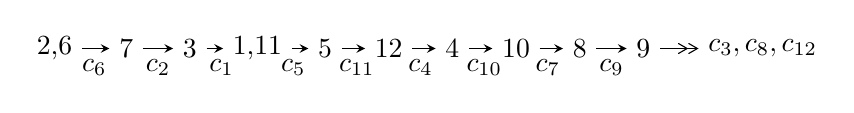
\begin{tikzpicture}[x=23pt, y=7pt]
	% node
	\node (A0) at (-1/8, 0) {2,6};
	\node (A1) at (1, 0) {7};
	\node (A2) at (2, 0) {3};
	\node (A3) at (49/16, 0) {1,11};
	\node (A4) at (33/8, 0) {5};
	\node (A5) at (41/8, 0) {12};
	\node (A6) at (49/8, 0) {4};
	\node (A7) at (57/8, 0) {10};
	\node (A8) at (65/8, 0) {8};
	\node (A9) at (73/8, 0) {9};
	\node (C1) at (1/2, -1) {$c_{6}$};
	\node (C2) at (3/2, -1) {$c_{2}$};
	\node (C3) at (5/2, -1) {$c_{1}$};
	\node (C4) at (29/8, -1) {$c_{5}$};
	\node (C5) at (37/8, -1) {$c_{11}$};
	\node (C6) at (45/8, -1) {$c_{4}$};
	\node (C7) at (53/8, -1) {$c_{10}$};
	\node (C8) at (61/8, -1) {$c_{7}$};
	\node (C9) at (69/8, -1) {$c_{9}$};
	\node (A10) at (11, 0) {$c_{3},c_{8},c_{12}$};

	% edge
	\draw[->,>=stealth]	
	(A0) edge (A1) (A1) edge (A2) (A2) edge (A3) (A3) edge (A4) (A4) edge (A5) (A5) edge (A6) (A6) edge (A7) (A7) edge (A8) (A8) edge (A9) ;
	\draw[->>,>={angle 60}]	
	(A9) edge (A10);
\end{tikzpicture} \\ 

\end{tabular} \\

\footnotetext{
The image of knot diagram is generated by the software ``\textbf{Draw programme}" developed by Andrew Bartholomew(\url{http://www.layer8.co.uk/maths/draw/index.htm\#Running-draw}), where we modified some parts for our purpose(\url{https://github.com/CATsTAILs/LinksPainter}).
}\phantom \\ \newline 
\centering \textbf{Ideals for irreducible components\footnotemark of $X_{\text{par}}$} 
 
\begin{align*}
I^u_{1}&=\langle 
-1.93763\times10^{105} u^{84}+6.40033\times10^{105} u^{83}+\cdots+5.22721\times10^{105} b-5.47893\times10^{106},\\
\phantom{I^u_{1}}&\phantom{= \langle  }-1.05688\times10^{107} u^{84}+1.58154\times10^{107} u^{83}+\cdots+9.93169\times10^{106} a+6.22411\times10^{108},\\
\phantom{I^u_{1}}&\phantom{= \langle  }u^{85}-2 u^{84}+\cdots-29 u+19\rangle \\
I^u_{2}&=\langle 
- u^{16}- u^{15}+\cdots+b-3,\\
\phantom{I^u_{2}}&\phantom{= \langle  }- u^{14}- u^{13}+3 u^{12}+2 u^{11}-8 u^{10}-4 u^9+12 u^8+3 u^7-15 u^6-3 u^5+12 u^4+u^3-5 u^2+a+2,\\
\phantom{I^u_{2}}&\phantom{= \langle  }u^{17}+u^{16}+\cdots+u+1\rangle \\
\\
\end{align*}
\raggedright * 2 irreducible components of $\dim_{\mathbb{C}}=0$, with total 102 representations.\\
\footnotetext{All coefficients of polynomials are rational numbers. But the coefficients are sometimes approximated in decimal forms when there is not enough margin.}
\newpage
\renewcommand{\arraystretch}{1}
\centering \section*{I. $I^u_{1}= \langle -1.94\times10^{105} u^{84}+6.40\times10^{105} u^{83}+\cdots+5.23\times10^{105} b-5.48\times10^{106},\;-1.06\times10^{107} u^{84}+1.58\times10^{107} u^{83}+\cdots+9.93\times10^{106} a+6.22\times10^{108},\;u^{85}-2 u^{84}+\cdots-29 u+19 \rangle$}
\flushleft \textbf{(i) Arc colorings}\\
\begin{tabular}{m{7pt} m{180pt} m{7pt} m{180pt} }
\flushright $a_{2}=$&$\begin{pmatrix}0\\u\end{pmatrix}$ \\
\flushright $a_{6}=$&$\begin{pmatrix}1\\0\end{pmatrix}$ \\
\flushright $a_{7}=$&$\begin{pmatrix}1\\u^2\end{pmatrix}$ \\
\flushright $a_{3}=$&$\begin{pmatrix}- u\\- u^3+u\end{pmatrix}$ \\
\flushright $a_{1}=$&$\begin{pmatrix}u^3\\u^5- u^3+u\end{pmatrix}$ \\
\flushright $a_{11}=$&$\begin{pmatrix}1.06415 u^{84}-1.59242 u^{83}+\cdots-9.71962 u-62.6691\\0.370682 u^{84}-1.22443 u^{83}+\cdots-53.3393 u+10.4816\end{pmatrix}$ \\
\flushright $a_{5}=$&$\begin{pmatrix}-0.366811 u^{84}-0.137769 u^{83}+\cdots-48.4547 u+21.4022\\-0.349390 u^{84}+0.613843 u^{83}+\cdots+15.4483 u+13.8709\end{pmatrix}$ \\
\flushright $a_{12}=$&$\begin{pmatrix}0.0586430 u^{84}+0.345218 u^{83}+\cdots-33.7770 u-4.01764\\-0.898344 u^{84}+2.16337 u^{83}+\cdots+76.0579 u-28.6076\end{pmatrix}$ \\
\flushright $a_{4}=$&$\begin{pmatrix}1.35820 u^{84}-1.82953 u^{83}+\cdots+44.0089 u-36.4802\\-0.879980 u^{84}+1.21621 u^{83}+\cdots+13.8302 u+15.4803\end{pmatrix}$ \\
\flushright $a_{10}=$&$\begin{pmatrix}1.43484 u^{84}-2.81684 u^{83}+\cdots-63.0589 u-52.1876\\0.370682 u^{84}-1.22443 u^{83}+\cdots-53.3393 u+10.4816\end{pmatrix}$ \\
\flushright $a_{8}=$&$\begin{pmatrix}0.861966 u^{84}-1.69287 u^{83}+\cdots+24.3927 u-72.7494\\-0.0526491 u^{84}+0.252680 u^{83}+\cdots-29.5740 u+4.29926\end{pmatrix}$ \\
\flushright $a_{9}=$&$\begin{pmatrix}1.28326 u^{84}-2.26001 u^{83}+\cdots-61.0116 u-45.5381\\0.329735 u^{84}-1.20748 u^{83}+\cdots-42.6117 u+13.5326\end{pmatrix}$\\&\end{tabular}
\flushleft \textbf{(ii) Obstruction class $= -1$}\\~\\
\flushleft \textbf{(iii) Cusp Shapes $= -0.130039 u^{84}+0.718141 u^{83}+\cdots+77.5891 u-93.5890$}\\~\\
\newpage\renewcommand{\arraystretch}{1}
\flushleft \textbf{(iv) u-Polynomials at the component}\newline \\
\begin{tabular}{m{50pt}|m{274pt}}
Crossings & \hspace{64pt}u-Polynomials at each crossing \\
\hline $$\begin{aligned}c_{1}\end{aligned}$$&$\begin{aligned}
&u^{85}+30 u^{84}+\cdots+17713 u+361
\end{aligned}$\\
\hline $$\begin{aligned}c_{2},c_{6}\end{aligned}$$&$\begin{aligned}
&u^{85}-2 u^{84}+\cdots-29 u+19
\end{aligned}$\\
\hline $$\begin{aligned}c_{3},c_{8}\end{aligned}$$&$\begin{aligned}
&u^{85}- u^{84}+\cdots+26 u+19
\end{aligned}$\\
\hline $$\begin{aligned}c_{4},c_{5},c_{10}\\c_{11}\end{aligned}$$&$\begin{aligned}
&u^{85}+u^{84}+\cdots-13 u+1
\end{aligned}$\\
\hline $$\begin{aligned}c_{7}\end{aligned}$$&$\begin{aligned}
&u^{85}-14 u^{84}+\cdots-548721 u+148409
\end{aligned}$\\
\hline $$\begin{aligned}c_{9}\end{aligned}$$&$\begin{aligned}
&u^{85}+4 u^{84}+\cdots+15735 u+2737
\end{aligned}$\\
\hline $$\begin{aligned}c_{12}\end{aligned}$$&$\begin{aligned}
&u^{85}-2 u^{84}+\cdots-405993 u+904999
\end{aligned}$\\
\hline
\end{tabular}\\~\\
\newpage\renewcommand{\arraystretch}{1}
\flushleft \textbf{(v) Riley Polynomials at the component}\newline \\
\begin{tabular}{m{50pt}|m{274pt}}
Crossings & \hspace{64pt}Riley Polynomials at each crossing \\
\hline $$\begin{aligned}c_{1}\end{aligned}$$&$\begin{aligned}
&y^{85}+58 y^{84}+\cdots+17060353 y-130321
\end{aligned}$\\
\hline $$\begin{aligned}c_{2},c_{6}\end{aligned}$$&$\begin{aligned}
&y^{85}-30 y^{84}+\cdots+17713 y-361
\end{aligned}$\\
\hline $$\begin{aligned}c_{3},c_{8}\end{aligned}$$&$\begin{aligned}
&y^{85}+77 y^{84}+\cdots-5556 y-361
\end{aligned}$\\
\hline $$\begin{aligned}c_{4},c_{5},c_{10}\\c_{11}\end{aligned}$$&$\begin{aligned}
&y^{85}+109 y^{84}+\cdots-127 y-1
\end{aligned}$\\
\hline $$\begin{aligned}c_{7}\end{aligned}$$&$\begin{aligned}
&y^{85}+36 y^{84}+\cdots-93911252195 y-22025231281
\end{aligned}$\\
\hline $$\begin{aligned}c_{9}\end{aligned}$$&$\begin{aligned}
&y^{85}+20 y^{84}+\cdots+4057439 y-7491169
\end{aligned}$\\
\hline $$\begin{aligned}c_{12}\end{aligned}$$&$\begin{aligned}
&y^{85}+44 y^{84}+\cdots-15920612859961 y-819023190001
\end{aligned}$\\
\hline
\end{tabular}\\~\\
\newpage\flushleft \textbf{(vi) Complex Volumes and Cusp Shapes}
$$\begin{array}{c|c|c}  
\text{Solutions to }I^u_{1}& \I (\text{vol} + \sqrt{-1}CS) & \text{Cusp shape}\\
 \hline 
\begin{aligned}
u &= \phantom{-}0.647105 + 0.753959 I \\
a &= -0.224133 - 0.420689 I \\
b &= \phantom{-}0.824332 - 0.180446 I\end{aligned}
 & \phantom{-}4.70008 + 2.71758 I & \phantom{-0.000000 } 0 \\ \hline\begin{aligned}
u &= \phantom{-}0.647105 - 0.753959 I \\
a &= -0.224133 + 0.420689 I \\
b &= \phantom{-}0.824332 + 0.180446 I\end{aligned}
 & \phantom{-}4.70008 - 2.71758 I & \phantom{-0.000000 } 0 \\ \hline\begin{aligned}
u &= -0.556564 + 0.860766 I \\
a &= -0.36210 - 2.15933 I \\
b &= \phantom{-}0.04521 + 1.67260 I\end{aligned}
 & \phantom{-}11.69870 + 0.50746 I & \phantom{-0.000000 } 0 \\ \hline\begin{aligned}
u &= -0.556564 - 0.860766 I \\
a &= -0.36210 + 2.15933 I \\
b &= \phantom{-}0.04521 - 1.67260 I\end{aligned}
 & \phantom{-}11.69870 - 0.50746 I & \phantom{-0.000000 } 0 \\ \hline\begin{aligned}
u &= -0.565073 + 0.787127 I \\
a &= -0.40557 + 2.28724 I \\
b &= -0.07092 - 1.67258 I\end{aligned}
 & \phantom{-}11.70450 - 3.80032 I & \phantom{-0.000000 } 0 \\ \hline\begin{aligned}
u &= -0.565073 - 0.787127 I \\
a &= -0.40557 - 2.28724 I \\
b &= -0.07092 + 1.67258 I\end{aligned}
 & \phantom{-}11.70450 + 3.80032 I & \phantom{-0.000000 } 0 \\ \hline\begin{aligned}
u &= -0.811348 + 0.652520 I \\
a &= -1.95108 - 1.86614 I \\
b &= \phantom{-}0.002056 + 0.816600 I\end{aligned}
 & \phantom{-}5.99934 + 0.54360 I & \phantom{-0.000000 } 0 \\ \hline\begin{aligned}
u &= -0.811348 - 0.652520 I \\
a &= -1.95108 + 1.86614 I \\
b &= \phantom{-}0.002056 - 0.816600 I\end{aligned}
 & \phantom{-}5.99934 - 0.54360 I & \phantom{-0.000000 } 0 \\ \hline\begin{aligned}
u &= -1.045990 + 0.023525 I \\
a &= \phantom{-}0.675867 + 0.404666 I \\
b &= \phantom{-}0.231608 + 0.627961 I\end{aligned}
 & -2.16388 - 1.62762 I & \phantom{-0.000000 } 0 \\ \hline\begin{aligned}
u &= -1.045990 - 0.023525 I \\
a &= \phantom{-}0.675867 - 0.404666 I \\
b &= \phantom{-}0.231608 - 0.627961 I\end{aligned}
 & -2.16388 + 1.62762 I & \phantom{-0.000000 } 0\\
 \hline 
 \end{array}$$\newpage$$\begin{array}{c|c|c}  
\text{Solutions to }I^u_{1}& \I (\text{vol} + \sqrt{-1}CS) & \text{Cusp shape}\\
 \hline 
\begin{aligned}
u &= -0.787091 + 0.701132 I \\
a &= \phantom{-}0.86089 + 1.51565 I \\
b &= \phantom{-}0.741333 - 0.874735 I\end{aligned}
 & \phantom{-}6.62681 + 2.54168 I & \phantom{-0.000000 } 0 \\ \hline\begin{aligned}
u &= -0.787091 - 0.701132 I \\
a &= \phantom{-}0.86089 - 1.51565 I \\
b &= \phantom{-}0.741333 + 0.874735 I\end{aligned}
 & \phantom{-}6.62681 - 2.54168 I & \phantom{-0.000000 } 0 \\ \hline\begin{aligned}
u &= \phantom{-}0.727290 + 0.600758 I \\
a &= -0.317175 + 0.570445 I \\
b &= \phantom{-}0.240056 - 0.954237 I\end{aligned}
 & \phantom{-}2.60222 - 1.41006 I & \phantom{-0.000000 } 0 \\ \hline\begin{aligned}
u &= \phantom{-}0.727290 - 0.600758 I \\
a &= -0.317175 - 0.570445 I \\
b &= \phantom{-}0.240056 + 0.954237 I\end{aligned}
 & \phantom{-}2.60222 + 1.41006 I & \phantom{-0.000000 } 0 \\ \hline\begin{aligned}
u &= -0.761116 + 0.550447 I \\
a &= -0.341801 - 0.103536 I \\
b &= -0.523133 - 0.083727 I\end{aligned}
 & \phantom{-}0.007740 + 0.354268 I & \phantom{-0.000000 } 0 \\ \hline\begin{aligned}
u &= -0.761116 - 0.550447 I \\
a &= -0.341801 + 0.103536 I \\
b &= -0.523133 + 0.083727 I\end{aligned}
 & \phantom{-}0.007740 - 0.354268 I & \phantom{-0.000000 } 0 \\ \hline\begin{aligned}
u &= -1.067980 + 0.060235 I \\
a &= -0.656023 + 0.333160 I \\
b &= -0.638161 - 0.121268 I\end{aligned}
 & -1.04027 + 2.23555 I & \phantom{-0.000000 } 0 \\ \hline\begin{aligned}
u &= -1.067980 - 0.060235 I \\
a &= -0.656023 - 0.333160 I \\
b &= -0.638161 + 0.121268 I\end{aligned}
 & -1.04027 - 2.23555 I & \phantom{-0.000000 } 0 \\ \hline\begin{aligned}
u &= \phantom{-}0.826055 + 0.686952 I \\
a &= -0.20738 + 3.33992 I \\
b &= -0.01217 - 1.69343 I\end{aligned}
 & \phantom{-}15.0313 - 4.7059 I & \phantom{-0.000000 } 0 \\ \hline\begin{aligned}
u &= \phantom{-}0.826055 - 0.686952 I \\
a &= -0.20738 - 3.33992 I \\
b &= -0.01217 + 1.69343 I\end{aligned}
 & \phantom{-}15.0313 + 4.7059 I & \phantom{-0.000000 } 0\\
 \hline 
 \end{array}$$\newpage$$\begin{array}{c|c|c}  
\text{Solutions to }I^u_{1}& \I (\text{vol} + \sqrt{-1}CS) & \text{Cusp shape}\\
 \hline 
\begin{aligned}
u &= \phantom{-}0.609980 + 0.679262 I \\
a &= -0.325099 - 1.045890 I \\
b &= -0.300819 + 0.858960 I\end{aligned}
 & \phantom{-}2.83585 + 2.41811 I & -12.00000 + 0. I\phantom{ +0.000000I} \\ \hline\begin{aligned}
u &= \phantom{-}0.609980 - 0.679262 I \\
a &= -0.325099 + 1.045890 I \\
b &= -0.300819 - 0.858960 I\end{aligned}
 & \phantom{-}2.83585 - 2.41811 I & -12.00000 + 0. I\phantom{ +0.000000I} \\ \hline\begin{aligned}
u &= -0.612018 + 0.899881 I \\
a &= -0.281445 - 1.092780 I \\
b &= \phantom{-}0.488638 + 1.001550 I\end{aligned}
 & \phantom{-}8.33566 - 7.04031 I & \phantom{-0.000000 } 0 \\ \hline\begin{aligned}
u &= -0.612018 - 0.899881 I \\
a &= -0.281445 + 1.092780 I \\
b &= \phantom{-}0.488638 - 1.001550 I\end{aligned}
 & \phantom{-}8.33566 + 7.04031 I & \phantom{-0.000000 } 0 \\ \hline\begin{aligned}
u &= \phantom{-}0.897868 + 0.155214 I \\
a &= \phantom{-}1.37373 - 0.80599 I \\
b &= \phantom{-}0.303749 + 0.272887 I\end{aligned}
 & -3.24400 - 0.43047 I & -16.2817 + 10.9205 I \\ \hline\begin{aligned}
u &= \phantom{-}0.897868 - 0.155214 I \\
a &= \phantom{-}1.37373 + 0.80599 I \\
b &= \phantom{-}0.303749 - 0.272887 I\end{aligned}
 & -3.24400 + 0.43047 I & -16.2817 - 10.9205 I \\ \hline\begin{aligned}
u &= -0.813594 + 0.405787 I \\
a &= \phantom{-}1.90281 + 1.78662 I \\
b &= \phantom{-}0.089790 - 1.372960 I\end{aligned}
 & \phantom{-}2.17807 + 1.68544 I & -12.00000 + 0. I\phantom{ +0.000000I} \\ \hline\begin{aligned}
u &= -0.813594 - 0.405787 I \\
a &= \phantom{-}1.90281 - 1.78662 I \\
b &= \phantom{-}0.089790 + 1.372960 I\end{aligned}
 & \phantom{-}2.17807 - 1.68544 I & -12.00000 + 0. I\phantom{ +0.000000I} \\ \hline\begin{aligned}
u &= -0.892941 + 0.643912 I \\
a &= \phantom{-}0.02925 - 2.05496 I \\
b &= -0.032718 + 0.920802 I\end{aligned}
 & \phantom{-}5.74174 + 4.50633 I & \phantom{-0.000000 } 0 \\ \hline\begin{aligned}
u &= -0.892941 - 0.643912 I \\
a &= \phantom{-}0.02925 + 2.05496 I \\
b &= -0.032718 - 0.920802 I\end{aligned}
 & \phantom{-}5.74174 - 4.50633 I & \phantom{-0.000000 } 0\\
 \hline 
 \end{array}$$\newpage$$\begin{array}{c|c|c}  
\text{Solutions to }I^u_{1}& \I (\text{vol} + \sqrt{-1}CS) & \text{Cusp shape}\\
 \hline 
\begin{aligned}
u &= \phantom{-}0.830217 + 0.723714 I \\
a &= \phantom{-}0.56953 - 2.00230 I \\
b &= -0.17837 + 1.75045 I\end{aligned}
 & \phantom{-}15.7652 + 0.8537 I & \phantom{-0.000000 } 0 \\ \hline\begin{aligned}
u &= \phantom{-}0.830217 - 0.723714 I \\
a &= \phantom{-}0.56953 + 2.00230 I \\
b &= -0.17837 - 1.75045 I\end{aligned}
 & \phantom{-}15.7652 - 0.8537 I & \phantom{-0.000000 } 0 \\ \hline\begin{aligned}
u &= \phantom{-}0.562524 + 0.698432 I \\
a &= -0.632069 + 0.699105 I \\
b &= \phantom{-}0.148063 + 0.105521 I\end{aligned}
 & \phantom{-}3.91125 - 0.86087 I & -7.44019 + 3.38376 I \\ \hline\begin{aligned}
u &= \phantom{-}0.562524 - 0.698432 I \\
a &= -0.632069 - 0.699105 I \\
b &= \phantom{-}0.148063 - 0.105521 I\end{aligned}
 & \phantom{-}3.91125 + 0.86087 I & -7.44019 - 3.38376 I \\ \hline\begin{aligned}
u &= -0.932054 + 0.609477 I \\
a &= \phantom{-}0.517583 + 0.527861 I \\
b &= \phantom{-}0.576720 + 0.064604 I\end{aligned}
 & -0.55714 + 4.33362 I & \phantom{-0.000000 } 0 \\ \hline\begin{aligned}
u &= -0.932054 - 0.609477 I \\
a &= \phantom{-}0.517583 - 0.527861 I \\
b &= \phantom{-}0.576720 - 0.064604 I\end{aligned}
 & -0.55714 - 4.33362 I & \phantom{-0.000000 } 0 \\ \hline\begin{aligned}
u &= \phantom{-}0.893893 + 0.681468 I \\
a &= -2.65625 + 2.64884 I \\
b &= -0.00283 - 1.67019 I\end{aligned}
 & \phantom{-}14.8209 - 0.5681 I & \phantom{-0.000000 } 0 \\ \hline\begin{aligned}
u &= \phantom{-}0.893893 - 0.681468 I \\
a &= -2.65625 - 2.64884 I \\
b &= -0.00283 + 1.67019 I\end{aligned}
 & \phantom{-}14.8209 + 0.5681 I & \phantom{-0.000000 } 0 \\ \hline\begin{aligned}
u &= \phantom{-}0.954964 + 0.633066 I \\
a &= -0.856249 + 0.886381 I \\
b &= -0.403009 - 0.741709 I\end{aligned}
 & \phantom{-}1.88427 - 3.52097 I & \phantom{-0.000000 } 0 \\ \hline\begin{aligned}
u &= \phantom{-}0.954964 - 0.633066 I \\
a &= -0.856249 - 0.886381 I \\
b &= -0.403009 + 0.741709 I\end{aligned}
 & \phantom{-}1.88427 + 3.52097 I & \phantom{-0.000000 } 0\\
 \hline 
 \end{array}$$\newpage$$\begin{array}{c|c|c}  
\text{Solutions to }I^u_{1}& \I (\text{vol} + \sqrt{-1}CS) & \text{Cusp shape}\\
 \hline 
\begin{aligned}
u &= \phantom{-}0.898469 + 0.713573 I \\
a &= \phantom{-}1.90554 - 1.88784 I \\
b &= \phantom{-}0.21178 + 1.71770 I\end{aligned}
 & \phantom{-}15.5555 - 6.3400 I & \phantom{-0.000000 } 0 \\ \hline\begin{aligned}
u &= \phantom{-}0.898469 - 0.713573 I \\
a &= \phantom{-}1.90554 + 1.88784 I \\
b &= \phantom{-}0.21178 - 1.71770 I\end{aligned}
 & \phantom{-}15.5555 + 6.3400 I & \phantom{-0.000000 } 0 \\ \hline\begin{aligned}
u &= -0.926032 + 0.681783 I \\
a &= \phantom{-}0.478596 + 0.485534 I \\
b &= -0.716859 - 0.982030 I\end{aligned}
 & \phantom{-}6.19768 + 2.77909 I & \phantom{-0.000000 } 0 \\ \hline\begin{aligned}
u &= -0.926032 - 0.681783 I \\
a &= \phantom{-}0.478596 - 0.485534 I \\
b &= -0.716859 + 0.982030 I\end{aligned}
 & \phantom{-}6.19768 - 2.77909 I & \phantom{-0.000000 } 0 \\ \hline\begin{aligned}
u &= -0.446139 + 1.072420 I \\
a &= -0.098836 + 0.989967 I \\
b &= \phantom{-}0.121122 - 0.860217 I\end{aligned}
 & \phantom{-}6.78292 + 1.92597 I & \phantom{-0.000000 } 0 \\ \hline\begin{aligned}
u &= -0.446139 - 1.072420 I \\
a &= -0.098836 - 0.989967 I \\
b &= \phantom{-}0.121122 + 0.860217 I\end{aligned}
 & \phantom{-}6.78292 - 1.92597 I & \phantom{-0.000000 } 0 \\ \hline\begin{aligned}
u &= \phantom{-}1.168160 + 0.042928 I \\
a &= \phantom{-}0.554142 + 0.148794 I \\
b &= \phantom{-}0.03344 + 1.61381 I\end{aligned}
 & \phantom{-}5.64367 - 2.43731 I & \phantom{-0.000000 } 0 \\ \hline\begin{aligned}
u &= \phantom{-}1.168160 - 0.042928 I \\
a &= \phantom{-}0.554142 - 0.148794 I \\
b &= \phantom{-}0.03344 - 1.61381 I\end{aligned}
 & \phantom{-}5.64367 + 2.43731 I & \phantom{-0.000000 } 0 \\ \hline\begin{aligned}
u &= \phantom{-}0.629848 + 0.994180 I \\
a &= -0.04602 + 2.25812 I \\
b &= \phantom{-}0.13524 - 1.71018 I\end{aligned}
 & \phantom{-}17.7707 + 9.5522 I & \phantom{-0.000000 } 0 \\ \hline\begin{aligned}
u &= \phantom{-}0.629848 - 0.994180 I \\
a &= -0.04602 - 2.25812 I \\
b &= \phantom{-}0.13524 + 1.71018 I\end{aligned}
 & \phantom{-}17.7707 - 9.5522 I & \phantom{-0.000000 } 0\\
 \hline 
 \end{array}$$\newpage$$\begin{array}{c|c|c}  
\text{Solutions to }I^u_{1}& \I (\text{vol} + \sqrt{-1}CS) & \text{Cusp shape}\\
 \hline 
\begin{aligned}
u &= \phantom{-}1.005390 + 0.647624 I \\
a &= \phantom{-}1.45289 - 1.00573 I \\
b &= \phantom{-}0.376561 + 0.808119 I\end{aligned}
 & \phantom{-}1.68859 - 7.58283 I & \phantom{-0.000000 } 0 \\ \hline\begin{aligned}
u &= \phantom{-}1.005390 - 0.647624 I \\
a &= \phantom{-}1.45289 + 1.00573 I \\
b &= \phantom{-}0.376561 - 0.808119 I\end{aligned}
 & \phantom{-}1.68859 + 7.58283 I & \phantom{-0.000000 } 0 \\ \hline\begin{aligned}
u &= -0.802068 + 0.045860 I \\
a &= -0.61059 - 1.85147 I \\
b &= \phantom{-}0.09331 - 1.61773 I\end{aligned}
 & \phantom{-}11.34640 + 2.99639 I & -8.69665 - 2.24681 I \\ \hline\begin{aligned}
u &= -0.802068 - 0.045860 I \\
a &= -0.61059 + 1.85147 I \\
b &= \phantom{-}0.09331 + 1.61773 I\end{aligned}
 & \phantom{-}11.34640 - 2.99639 I & -8.69665 + 2.24681 I \\ \hline\begin{aligned}
u &= \phantom{-}0.789258 + 0.059653 I \\
a &= -1.103960 + 0.847330 I \\
b &= -0.328099 - 1.040420 I\end{aligned}
 & \phantom{-}2.55734 - 1.18348 I & -8.52720 + 1.71025 I \\ \hline\begin{aligned}
u &= \phantom{-}0.789258 - 0.059653 I \\
a &= -1.103960 - 0.847330 I \\
b &= -0.328099 + 1.040420 I\end{aligned}
 & \phantom{-}2.55734 + 1.18348 I & -8.52720 - 1.71025 I \\ \hline\begin{aligned}
u &= \phantom{-}1.012580 + 0.685568 I \\
a &= -0.181393 + 0.667802 I \\
b &= -0.898129 - 0.088432 I\end{aligned}
 & \phantom{-}3.61303 - 8.20470 I & \phantom{-0.000000 } 0 \\ \hline\begin{aligned}
u &= \phantom{-}1.012580 - 0.685568 I \\
a &= -0.181393 - 0.667802 I \\
b &= -0.898129 + 0.088432 I\end{aligned}
 & \phantom{-}3.61303 + 8.20470 I & \phantom{-0.000000 } 0 \\ \hline\begin{aligned}
u &= \phantom{-}1.037250 + 0.662366 I \\
a &= \phantom{-}0.345822 + 0.438701 I \\
b &= \phantom{-}0.0335953 - 0.1026880 I\end{aligned}
 & \phantom{-}2.54217 - 4.42223 I & \phantom{-0.000000 } 0 \\ \hline\begin{aligned}
u &= \phantom{-}1.037250 - 0.662366 I \\
a &= \phantom{-}0.345822 - 0.438701 I \\
b &= \phantom{-}0.0335953 + 0.1026880 I\end{aligned}
 & \phantom{-}2.54217 + 4.42223 I & \phantom{-0.000000 } 0\\
 \hline 
 \end{array}$$\newpage$$\begin{array}{c|c|c}  
\text{Solutions to }I^u_{1}& \I (\text{vol} + \sqrt{-1}CS) & \text{Cusp shape}\\
 \hline 
\begin{aligned}
u &= \phantom{-}1.228980 + 0.203243 I \\
a &= -0.536826 + 0.200839 I \\
b &= -0.420598 - 0.753985 I\end{aligned}
 & \phantom{-}0.87355 - 5.82145 I & \phantom{-0.000000 } 0 \\ \hline\begin{aligned}
u &= \phantom{-}1.228980 - 0.203243 I \\
a &= -0.536826 - 0.200839 I \\
b &= -0.420598 + 0.753985 I\end{aligned}
 & \phantom{-}0.87355 + 5.82145 I & \phantom{-0.000000 } 0 \\ \hline\begin{aligned}
u &= -1.049270 + 0.676448 I \\
a &= \phantom{-}2.33788 + 1.53668 I \\
b &= \phantom{-}0.09332 - 1.66009 I\end{aligned}
 & \phantom{-}10.28640 + 9.32446 I & \phantom{-0.000000 } 0 \\ \hline\begin{aligned}
u &= -1.049270 - 0.676448 I \\
a &= \phantom{-}2.33788 - 1.53668 I \\
b &= \phantom{-}0.09332 + 1.66009 I\end{aligned}
 & \phantom{-}10.28640 - 9.32446 I & \phantom{-0.000000 } 0 \\ \hline\begin{aligned}
u &= -1.071800 + 0.726814 I \\
a &= -1.01750 - 1.29587 I \\
b &= -0.566947 + 0.990313 I\end{aligned}
 & \phantom{-}6.9269 + 13.0405 I & \phantom{-0.000000 } 0 \\ \hline\begin{aligned}
u &= -1.071800 - 0.726814 I \\
a &= -1.01750 + 1.29587 I \\
b &= -0.566947 - 0.990313 I\end{aligned}
 & \phantom{-}6.9269 - 13.0405 I & \phantom{-0.000000 } 0 \\ \hline\begin{aligned}
u &= -1.087270 + 0.727678 I \\
a &= -1.41199 - 1.55195 I \\
b &= -0.10415 + 1.64080 I\end{aligned}
 & \phantom{-}10.13050 + 5.39662 I & \phantom{-0.000000 } 0 \\ \hline\begin{aligned}
u &= -1.087270 - 0.727678 I \\
a &= -1.41199 + 1.55195 I \\
b &= -0.10415 - 1.64080 I\end{aligned}
 & \phantom{-}10.13050 - 5.39662 I & \phantom{-0.000000 } 0 \\ \hline\begin{aligned}
u &= \phantom{-}0.472230 + 1.259750 I \\
a &= \phantom{-}0.13075 - 2.11971 I \\
b &= \phantom{-}0.02922 + 1.67563 I\end{aligned}
 & \phantom{-}15.7426 - 2.4908 I & \phantom{-0.000000 } 0 \\ \hline\begin{aligned}
u &= \phantom{-}0.472230 - 1.259750 I \\
a &= \phantom{-}0.13075 + 2.11971 I \\
b &= \phantom{-}0.02922 - 1.67563 I\end{aligned}
 & \phantom{-}15.7426 + 2.4908 I & \phantom{-0.000000 } 0\\
 \hline 
 \end{array}$$\newpage$$\begin{array}{c|c|c}  
\text{Solutions to }I^u_{1}& \I (\text{vol} + \sqrt{-1}CS) & \text{Cusp shape}\\
 \hline 
\begin{aligned}
u &= \phantom{-}1.107400 + 0.767076 I \\
a &= -1.75743 + 1.77279 I \\
b &= -0.16023 - 1.71067 I\end{aligned}
 & \phantom{-}16.2658 - 15.9591 I & \phantom{-0.000000 } 0 \\ \hline\begin{aligned}
u &= \phantom{-}1.107400 - 0.767076 I \\
a &= -1.75743 - 1.77279 I \\
b &= -0.16023 + 1.71067 I\end{aligned}
 & \phantom{-}16.2658 + 15.9591 I & \phantom{-0.000000 } 0 \\ \hline\begin{aligned}
u &= \phantom{-}0.551963 + 0.313389 I \\
a &= -0.964569 + 0.755921 I \\
b &= -0.066335 - 1.023540 I\end{aligned}
 & \phantom{-}2.38998 - 1.32990 I & -6.70793 + 4.87191 I \\ \hline\begin{aligned}
u &= \phantom{-}0.551963 - 0.313389 I \\
a &= -0.964569 - 0.755921 I \\
b &= -0.066335 + 1.023540 I\end{aligned}
 & \phantom{-}2.38998 + 1.32990 I & -6.70793 - 4.87191 I \\ \hline\begin{aligned}
u &= -1.152350 + 0.798898 I \\
a &= \phantom{-}0.770641 + 0.797164 I \\
b &= \phantom{-}0.045398 - 0.819870 I\end{aligned}
 & \phantom{-}4.70193 + 4.76066 I & \phantom{-0.000000 } 0 \\ \hline\begin{aligned}
u &= -1.152350 - 0.798898 I \\
a &= \phantom{-}0.770641 - 0.797164 I \\
b &= \phantom{-}0.045398 + 0.819870 I\end{aligned}
 & \phantom{-}4.70193 - 4.76066 I & \phantom{-0.000000 } 0 \\ \hline\begin{aligned}
u &= -1.380490 + 0.277313 I \\
a &= -0.656547 - 0.660540 I \\
b &= -0.09664 + 1.64151 I\end{aligned}
 & \phantom{-}9.14952 + 7.66751 I & \phantom{-0.000000 } 0 \\ \hline\begin{aligned}
u &= -1.380490 - 0.277313 I \\
a &= -0.656547 + 0.660540 I \\
b &= -0.09664 - 1.64151 I\end{aligned}
 & \phantom{-}9.14952 - 7.66751 I & \phantom{-0.000000 } 0 \\ \hline\begin{aligned}
u &= -0.563721 + 0.067562 I \\
a &= -1.40491 + 1.49605 I \\
b &= -0.06817 - 1.70836 I\end{aligned}
 & \phantom{-}12.20380 - 2.58863 I & -11.77943 + 3.33602 I \\ \hline\begin{aligned}
u &= -0.563721 - 0.067562 I \\
a &= -1.40491 - 1.49605 I \\
b &= -0.06817 + 1.70836 I\end{aligned}
 & \phantom{-}12.20380 + 2.58863 I & -11.77943 - 3.33602 I\\
 \hline 
 \end{array}$$\newpage$$\begin{array}{c|c|c}  
\text{Solutions to }I^u_{1}& \I (\text{vol} + \sqrt{-1}CS) & \text{Cusp shape}\\
 \hline 
\begin{aligned}
u &= \phantom{-}1.21378 + 0.87933 I \\
a &= \phantom{-}1.10685 - 1.70532 I \\
b &= \phantom{-}0.01240 + 1.66995 I\end{aligned}
 & \phantom{-}13.5267 - 4.9848 I & \phantom{-0.000000 } 0 \\ \hline\begin{aligned}
u &= \phantom{-}1.21378 - 0.87933 I \\
a &= \phantom{-}1.10685 + 1.70532 I \\
b &= \phantom{-}0.01240 - 1.66995 I\end{aligned}
 & \phantom{-}13.5267 + 4.9848 I & \phantom{-0.000000 } 0 \\ \hline\begin{aligned}
u &= \phantom{-}0.414901 + 0.112651 I \\
a &= -0.19032 + 3.03332 I \\
b &= \phantom{-}0.365746 + 0.532815 I\end{aligned}
 & \phantom{-}3.75166 - 1.38468 I & -10.94065 + 4.57640 I \\ \hline\begin{aligned}
u &= \phantom{-}0.414901 - 0.112651 I \\
a &= -0.19032 - 3.03332 I \\
b &= \phantom{-}0.365746 - 0.532815 I\end{aligned}
 & \phantom{-}3.75166 + 1.38468 I & -10.94065 - 4.57640 I \\ \hline\begin{aligned}
u &= -0.310404\phantom{ +0.000000I} \\
a &= -0.683642\phantom{ +0.000000I} \\
b &= -0.308825\phantom{ +0.000000I}\end{aligned}
 & -0.534005\phantom{ +0.000000I} & -18.4650\phantom{ +0.000000I}\\
 \hline 
 \end{array}$$\newpage\newpage\renewcommand{\arraystretch}{1}
\centering \section*{II. $I^u_{2}= \langle - u^{16}- u^{15}+\cdots+b-3,\;- u^{14}- u^{13}+\cdots+a+2,\;u^{17}+u^{16}+\cdots+u+1 \rangle$}
\flushleft \textbf{(i) Arc colorings}\\
\begin{tabular}{m{7pt} m{180pt} m{7pt} m{180pt} }
\flushright $a_{2}=$&$\begin{pmatrix}0\\u\end{pmatrix}$ \\
\flushright $a_{6}=$&$\begin{pmatrix}1\\0\end{pmatrix}$ \\
\flushright $a_{7}=$&$\begin{pmatrix}1\\u^2\end{pmatrix}$ \\
\flushright $a_{3}=$&$\begin{pmatrix}- u\\- u^3+u\end{pmatrix}$ \\
\flushright $a_{1}=$&$\begin{pmatrix}u^3\\u^5- u^3+u\end{pmatrix}$ \\
\flushright $a_{11}=$&$\begin{pmatrix}u^{14}+u^{13}+\cdots+5 u^2-2\\u^{16}+u^{15}+\cdots-10 u^2+3\end{pmatrix}$ \\
\flushright $a_{5}=$&$\begin{pmatrix}- u^{13}- u^{12}+2 u^{11}+2 u^{10}-5 u^9-4 u^8+4 u^7+3 u^6-5 u^5-3 u^4+u^3+u^2\\-2 u^{16}- u^{15}+\cdots+6 u^2-2 u\end{pmatrix}$ \\
\flushright $a_{12}=$&$\begin{pmatrix}- u^{16}- u^{15}+\cdots+u-1\\-2 u^{16}-2 u^{15}+\cdots+2 u-4\end{pmatrix}$ \\
\flushright $a_{4}=$&$\begin{pmatrix}u^{14}-3 u^{12}+7 u^{10}- u^9-9 u^8+u^7+10 u^6-2 u^5-7 u^4- u^3+3 u^2+u-1\\3 u^{16}+u^{15}+\cdots+3 u+2\end{pmatrix}$ \\
\flushright $a_{10}=$&$\begin{pmatrix}u^{16}+u^{15}+\cdots-5 u^2+1\\u^{16}+u^{15}+\cdots-10 u^2+3\end{pmatrix}$ \\
\flushright $a_{8}=$&$\begin{pmatrix}- u^4+u^2-1\\u^{16}- u^{15}+\cdots+3 u-1\end{pmatrix}$ \\
\flushright $a_{9}=$&$\begin{pmatrix}u^{16}-3 u^{14}+\cdots+u+1\\u^{16}+u^{15}+\cdots-9 u^2+3\end{pmatrix}$\\&\end{tabular}
\flushleft \textbf{(ii) Obstruction class $= 1$}\\~\\
\flushleft \textbf{(iii) Cusp Shapes $= -2 u^{16}+5 u^{15}+11 u^{14}-14 u^{13}-28 u^{12}+38 u^{11}+47 u^{10}-53 u^9-58 u^8+68 u^7+52 u^6-51 u^5-40 u^4+26 u^3+16 u^2-12 u-11$}\\~\\
\newpage\renewcommand{\arraystretch}{1}
\flushleft \textbf{(iv) u-Polynomials at the component}\newline \\
\begin{tabular}{m{50pt}|m{274pt}}
Crossings & \hspace{64pt}u-Polynomials at each crossing \\
\hline $$\begin{aligned}c_{1}\end{aligned}$$&$\begin{aligned}
&u^{17}-7 u^{16}+\cdots+7 u-1
\end{aligned}$\\
\hline $$\begin{aligned}c_{2}\end{aligned}$$&$\begin{aligned}
&u^{17}- u^{16}+\cdots+u-1
\end{aligned}$\\
\hline $$\begin{aligned}c_{3}\end{aligned}$$&$\begin{aligned}
&u^{17}+10 u^{15}+\cdots+4 u-3
\end{aligned}$\\
\hline $$\begin{aligned}c_{4},c_{5}\end{aligned}$$&$\begin{aligned}
&u^{17}+12 u^{15}+\cdots+7 u+1
\end{aligned}$\\
\hline $$\begin{aligned}c_{6}\end{aligned}$$&$\begin{aligned}
&u^{17}+u^{16}+\cdots+u+1
\end{aligned}$\\
\hline $$\begin{aligned}c_{7}\end{aligned}$$&$\begin{aligned}
&u^{17}+3 u^{16}+\cdots-3 u-1
\end{aligned}$\\
\hline $$\begin{aligned}c_{8}\end{aligned}$$&$\begin{aligned}
&u^{17}+10 u^{15}+\cdots+4 u+3
\end{aligned}$\\
\hline $$\begin{aligned}c_{9}\end{aligned}$$&$\begin{aligned}
&u^{17}+3 u^{16}+\cdots+u-1
\end{aligned}$\\
\hline $$\begin{aligned}c_{10},c_{11}\end{aligned}$$&$\begin{aligned}
&u^{17}+12 u^{15}+\cdots+7 u-1
\end{aligned}$\\
\hline $$\begin{aligned}c_{12}\end{aligned}$$&$\begin{aligned}
&u^{17}+u^{16}+\cdots-3 u+1
\end{aligned}$\\
\hline
\end{tabular}\\~\\
\newpage\renewcommand{\arraystretch}{1}
\flushleft \textbf{(v) Riley Polynomials at the component}\newline \\
\begin{tabular}{m{50pt}|m{274pt}}
Crossings & \hspace{64pt}Riley Polynomials at each crossing \\
\hline $$\begin{aligned}c_{1}\end{aligned}$$&$\begin{aligned}
&y^{17}+13 y^{16}+\cdots-13 y-1
\end{aligned}$\\
\hline $$\begin{aligned}c_{2},c_{6}\end{aligned}$$&$\begin{aligned}
&y^{17}-7 y^{16}+\cdots+7 y-1
\end{aligned}$\\
\hline $$\begin{aligned}c_{3},c_{8}\end{aligned}$$&$\begin{aligned}
&y^{17}+20 y^{16}+\cdots+10 y-9
\end{aligned}$\\
\hline $$\begin{aligned}c_{4},c_{5},c_{10}\\c_{11}\end{aligned}$$&$\begin{aligned}
&y^{17}+24 y^{16}+\cdots+35 y-1
\end{aligned}$\\
\hline $$\begin{aligned}c_{7}\end{aligned}$$&$\begin{aligned}
&y^{17}+3 y^{16}+\cdots- y-1
\end{aligned}$\\
\hline $$\begin{aligned}c_{9}\end{aligned}$$&$\begin{aligned}
&y^{17}- y^{16}+\cdots-3 y-1
\end{aligned}$\\
\hline $$\begin{aligned}c_{12}\end{aligned}$$&$\begin{aligned}
&y^{17}+3 y^{16}+\cdots+y-1
\end{aligned}$\\
\hline
\end{tabular}\\~\\
\newpage\flushleft \textbf{(vi) Complex Volumes and Cusp Shapes}
$$\begin{array}{c|c|c}  
\text{Solutions to }I^u_{2}& \I (\text{vol} + \sqrt{-1}CS) & \text{Cusp shape}\\
 \hline 
\begin{aligned}
u &= -0.720152 + 0.656706 I \\
a &= \phantom{-}0.79944 + 1.95784 I \\
b &= \phantom{-}0.319931 - 0.860450 I\end{aligned}
 & \phantom{-}5.06979 + 2.15267 I & -5.68896 - 4.26478 I \\ \hline\begin{aligned}
u &= -0.720152 - 0.656706 I \\
a &= \phantom{-}0.79944 - 1.95784 I \\
b &= \phantom{-}0.319931 + 0.860450 I\end{aligned}
 & \phantom{-}5.06979 - 2.15267 I & -5.68896 + 4.26478 I \\ \hline\begin{aligned}
u &= \phantom{-}0.844913 + 0.200306 I \\
a &= -1.65011 + 0.63197 I \\
b &= -0.092358 - 1.290120 I\end{aligned}
 & \phantom{-}1.30360 - 0.87814 I & -15.0870 - 0.5641 I \\ \hline\begin{aligned}
u &= \phantom{-}0.844913 - 0.200306 I \\
a &= -1.65011 - 0.63197 I \\
b &= -0.092358 + 1.290120 I\end{aligned}
 & \phantom{-}1.30360 + 0.87814 I & -15.0870 + 0.5641 I \\ \hline\begin{aligned}
u &= -0.862236\phantom{ +0.000000I} \\
a &= -1.51495\phantom{ +0.000000I} \\
b &= -0.147176\phantom{ +0.000000I}\end{aligned}
 & -2.99854\phantom{ +0.000000I} & -8.51500\phantom{ +0.000000I} \\ \hline\begin{aligned}
u &= \phantom{-}0.776801 + 0.839562 I \\
a &= \phantom{-}0.78100 - 2.66977 I \\
b &= \phantom{-}0.02762 + 1.69581 I\end{aligned}
 & \phantom{-}14.4535 - 3.1568 I & -3.79045 + 2.68402 I \\ \hline\begin{aligned}
u &= \phantom{-}0.776801 - 0.839562 I \\
a &= \phantom{-}0.78100 + 2.66977 I \\
b &= \phantom{-}0.02762 - 1.69581 I\end{aligned}
 & \phantom{-}14.4535 + 3.1568 I & -3.79045 - 2.68402 I \\ \hline\begin{aligned}
u &= -0.942687 + 0.675044 I \\
a &= \phantom{-}0.574582 + 0.958429 I \\
b &= -0.246755 - 1.006550 I\end{aligned}
 & \phantom{-}4.37714 + 3.08094 I & -6.66676 - 2.63554 I \\ \hline\begin{aligned}
u &= -0.942687 - 0.675044 I \\
a &= \phantom{-}0.574582 - 0.958429 I \\
b &= -0.246755 + 1.006550 I\end{aligned}
 & \phantom{-}4.37714 - 3.08094 I & -6.66676 + 2.63554 I \\ \hline\begin{aligned}
u &= \phantom{-}0.626628 + 0.526088 I \\
a &= \phantom{-}0.105161 - 0.770507 I \\
b &= \phantom{-}0.374391 - 0.661733 I\end{aligned}
 & \phantom{-}4.43105 + 0.41822 I & -4.85621 - 0.33566 I\\
 \hline 
 \end{array}$$\newpage$$\begin{array}{c|c|c}  
\text{Solutions to }I^u_{2}& \I (\text{vol} + \sqrt{-1}CS) & \text{Cusp shape}\\
 \hline 
\begin{aligned}
u &= \phantom{-}0.626628 - 0.526088 I \\
a &= \phantom{-}0.105161 + 0.770507 I \\
b &= \phantom{-}0.374391 + 0.661733 I\end{aligned}
 & \phantom{-}4.43105 - 0.41822 I & -4.85621 + 0.33566 I \\ \hline\begin{aligned}
u &= \phantom{-}1.084210 + 0.640691 I \\
a &= -0.553437 + 0.314492 I \\
b &= -0.309644 - 0.517094 I\end{aligned}
 & \phantom{-}2.82046 - 5.17696 I & -5.91305 + 8.94380 I \\ \hline\begin{aligned}
u &= \phantom{-}1.084210 - 0.640691 I \\
a &= -0.553437 - 0.314492 I \\
b &= -0.309644 + 0.517094 I\end{aligned}
 & \phantom{-}2.82046 + 5.17696 I & -5.91305 - 8.94380 I \\ \hline\begin{aligned}
u &= -0.541603 + 0.427521 I \\
a &= -0.051956 - 0.620358 I \\
b &= \phantom{-}0.09256 + 1.67798 I\end{aligned}
 & \phantom{-}12.88990 - 2.20254 I & -1.59840 - 1.45365 I \\ \hline\begin{aligned}
u &= -0.541603 - 0.427521 I \\
a &= -0.051956 + 0.620358 I \\
b &= \phantom{-}0.09256 - 1.67798 I\end{aligned}
 & \phantom{-}12.88990 + 2.20254 I & -1.59840 + 1.45365 I \\ \hline\begin{aligned}
u &= -1.196990 + 0.623400 I \\
a &= -1.24721 - 0.98437 I \\
b &= -0.09216 + 1.61922 I\end{aligned}
 & \phantom{-}10.43660 + 6.68767 I & -4.14164 - 6.03567 I \\ \hline\begin{aligned}
u &= -1.196990 - 0.623400 I \\
a &= -1.24721 + 0.98437 I \\
b &= -0.09216 - 1.61922 I\end{aligned}
 & \phantom{-}10.43660 - 6.68767 I & -4.14164 + 6.03567 I\\
 \hline 
 \end{array}$$\newpage
\newpage\renewcommand{\arraystretch}{1}
\centering \section*{ III. u-Polynomials}
\begin{tabular}{m{50pt}|m{274pt}}
Crossings & \hspace{64pt}u-Polynomials at each crossing \\
\hline $$\begin{aligned}c_{1}\end{aligned}$$&$\begin{aligned}
&(u^{17}-7 u^{16}+\cdots+7 u-1)(u^{85}+30 u^{84}+\cdots+17713 u+361)
\end{aligned}$\\
\hline $$\begin{aligned}c_{2}\end{aligned}$$&$\begin{aligned}
&(u^{17}- u^{16}+\cdots+u-1)(u^{85}-2 u^{84}+\cdots-29 u+19)
\end{aligned}$\\
\hline $$\begin{aligned}c_{3}\end{aligned}$$&$\begin{aligned}
&(u^{17}+10 u^{15}+\cdots+4 u-3)(u^{85}- u^{84}+\cdots+26 u+19)
\end{aligned}$\\
\hline $$\begin{aligned}c_{4},c_{5}\end{aligned}$$&$\begin{aligned}
&(u^{17}+12 u^{15}+\cdots+7 u+1)(u^{85}+u^{84}+\cdots-13 u+1)
\end{aligned}$\\
\hline $$\begin{aligned}c_{6}\end{aligned}$$&$\begin{aligned}
&(u^{17}+u^{16}+\cdots+u+1)(u^{85}-2 u^{84}+\cdots-29 u+19)
\end{aligned}$\\
\hline $$\begin{aligned}c_{7}\end{aligned}$$&$\begin{aligned}
&(u^{17}+3 u^{16}+\cdots-3 u-1)(u^{85}-14 u^{84}+\cdots-548721 u+148409)
\end{aligned}$\\
\hline $$\begin{aligned}c_{8}\end{aligned}$$&$\begin{aligned}
&(u^{17}+10 u^{15}+\cdots+4 u+3)(u^{85}- u^{84}+\cdots+26 u+19)
\end{aligned}$\\
\hline $$\begin{aligned}c_{9}\end{aligned}$$&$\begin{aligned}
&(u^{17}+3 u^{16}+\cdots+u-1)(u^{85}+4 u^{84}+\cdots+15735 u+2737)
\end{aligned}$\\
\hline $$\begin{aligned}c_{10},c_{11}\end{aligned}$$&$\begin{aligned}
&(u^{17}+12 u^{15}+\cdots+7 u-1)(u^{85}+u^{84}+\cdots-13 u+1)
\end{aligned}$\\
\hline $$\begin{aligned}c_{12}\end{aligned}$$&$\begin{aligned}
&(u^{17}+u^{16}+\cdots-3 u+1)(u^{85}-2 u^{84}+\cdots-405993 u+904999)
\end{aligned}$\\
\hline
\end{tabular}\newpage\renewcommand{\arraystretch}{1}
\centering \section*{ IV. Riley Polynomials}
\begin{tabular}{m{50pt}|m{274pt}}
Crossings & \hspace{64pt}Riley Polynomials at each crossing \\
\hline $$\begin{aligned}c_{1}\end{aligned}$$&$\begin{aligned}
&(y^{17}+13 y^{16}+\cdots-13 y-1)\\
&\cdot(y^{85}+58 y^{84}+\cdots+17060353 y-130321)
\end{aligned}$\\
\hline $$\begin{aligned}c_{2},c_{6}\end{aligned}$$&$\begin{aligned}
&(y^{17}-7 y^{16}+\cdots+7 y-1)(y^{85}-30 y^{84}+\cdots+17713 y-361)
\end{aligned}$\\
\hline $$\begin{aligned}c_{3},c_{8}\end{aligned}$$&$\begin{aligned}
&(y^{17}+20 y^{16}+\cdots+10 y-9)(y^{85}+77 y^{84}+\cdots-5556 y-361)
\end{aligned}$\\
\hline $$\begin{aligned}c_{4},c_{5},c_{10}\\c_{11}\end{aligned}$$&$\begin{aligned}
&(y^{17}+24 y^{16}+\cdots+35 y-1)(y^{85}+109 y^{84}+\cdots-127 y-1)
\end{aligned}$\\
\hline $$\begin{aligned}c_{7}\end{aligned}$$&$\begin{aligned}
&(y^{17}+3 y^{16}+\cdots- y-1)\\
&\cdot(y^{85}+36 y^{84}+\cdots-93911252195 y-22025231281)
\end{aligned}$\\
\hline $$\begin{aligned}c_{9}\end{aligned}$$&$\begin{aligned}
&(y^{17}- y^{16}+\cdots-3 y-1)(y^{85}+20 y^{84}+\cdots+4057439 y-7491169)
\end{aligned}$\\
\hline $$\begin{aligned}c_{12}\end{aligned}$$&$\begin{aligned}
&(y^{17}+3 y^{16}+\cdots+y-1)\\
&\cdot(y^{85}+44 y^{84}+\cdots-15920612859961 y-819023190001)
\end{aligned}$\\
\hline
\end{tabular}
\vskip 2pc
\end{document}